% vim: spelllang=cs spell textwidth=120
\documentclass{beamer}
\usepackage[czech]{babel}
\definecolor{links}{HTML}{2A1B81}
\usepackage[utf8]{inputenc}
%\usepackage{ucs}
%\usepackage[utf8x]{inputenc}
\usepackage{minted}
\usepackage{hyperref}
\usepackage[overlay]{textpos}
\hypersetup{colorlinks,urlcolor=links}
\setbeamertemplate{navigation symbols}{}

\begin{document}

\title{Deska: Tool for Central Administration of a Grid Site}
\author{Jan Kundrát \\ \href{mailto:kundratj@fzu.cz}{\nolinkurl{kundratj@fzu.cz}}
\vspace{5mm}
\\ Lukáš Kerpl \\ Martina Krejčová \\ Tomáš Hubík}
\institute{Institute of Physics of the AS CR, v.v.i.}
\begin{frame}
\begin{columns}
\begin{column}{.4\textwidth}

\includegraphics[width=4cm]{../HEPIX-2011/logo-FZU-male.pdf} \\

\includegraphics[width=4cm]{../HEPIX-2011/deska_logo.pdf}
\end{column}
\begin{column}{.6\textwidth}
\maketitle
\end{column}
\end{columns}
\end{frame}


\begin{frame}[fragile]
\frametitle{Úvod: FZÚ AV ČR, v.v.i.}
\begin{itemize}
    \item 350 serverů, 3000~CPU, 2~PB HDD, $n\times$10~Gb konektivita
        \begin{itemize}
            \item spolupráce s~CERN
            \item analýza dat z urychlovače LHC
            \item experiment D0, Fermilab, USA
            \item jedno z~nejrozsáhlejších výpočetních center v~ČR
        \end{itemize}
\end{itemize}
\end{frame}


\begin{frame}[fragile]
\frametitle{Problém: duplicitní informace}
\begin{itemize}
    \item Informace o každém serveru / službě rozprostřena po celé infrastruktuře
        \begin{itemize}
            \item HW DB
            \item síťové přepínače
            \item DHCP
            \item DNS
            \item specifikace rolí v~Cfengine
            \item Torque a CPU multiplikátory
            \item MRTG \& RRD grafování
            \item Nagios
            \item Ganglia
            \item Munin
            \item \ldots
        \end{itemize}
    \item Komplikované změny, časté omyly, zdroj komplikací
\end{itemize}
\end{frame}


\begin{frame}[fragile]
\frametitle{Navrhované řešení}
\begin{columns}
\begin{column}{.45\paperwidth}
    \begin{itemize}
        \item Jedno centrální místo jako autoritativní zdroj informací
        \item Provádění změn:
            \begin{enumerate}
                \item Změna dat v~DB
                \item Vygenerování výstupu
                \item Kontrola změn
                \item Uložení k~distribuci
                \item Nasazení do praxe
            \end{enumerate}
        \item Neschválené změny neovlivňují další uživatele ani stav produkčních systémů
    \end{itemize}
\end{column}
\begin{column}{.55\paperwidth}
\begin{textblock}{50}(0,-7.2)
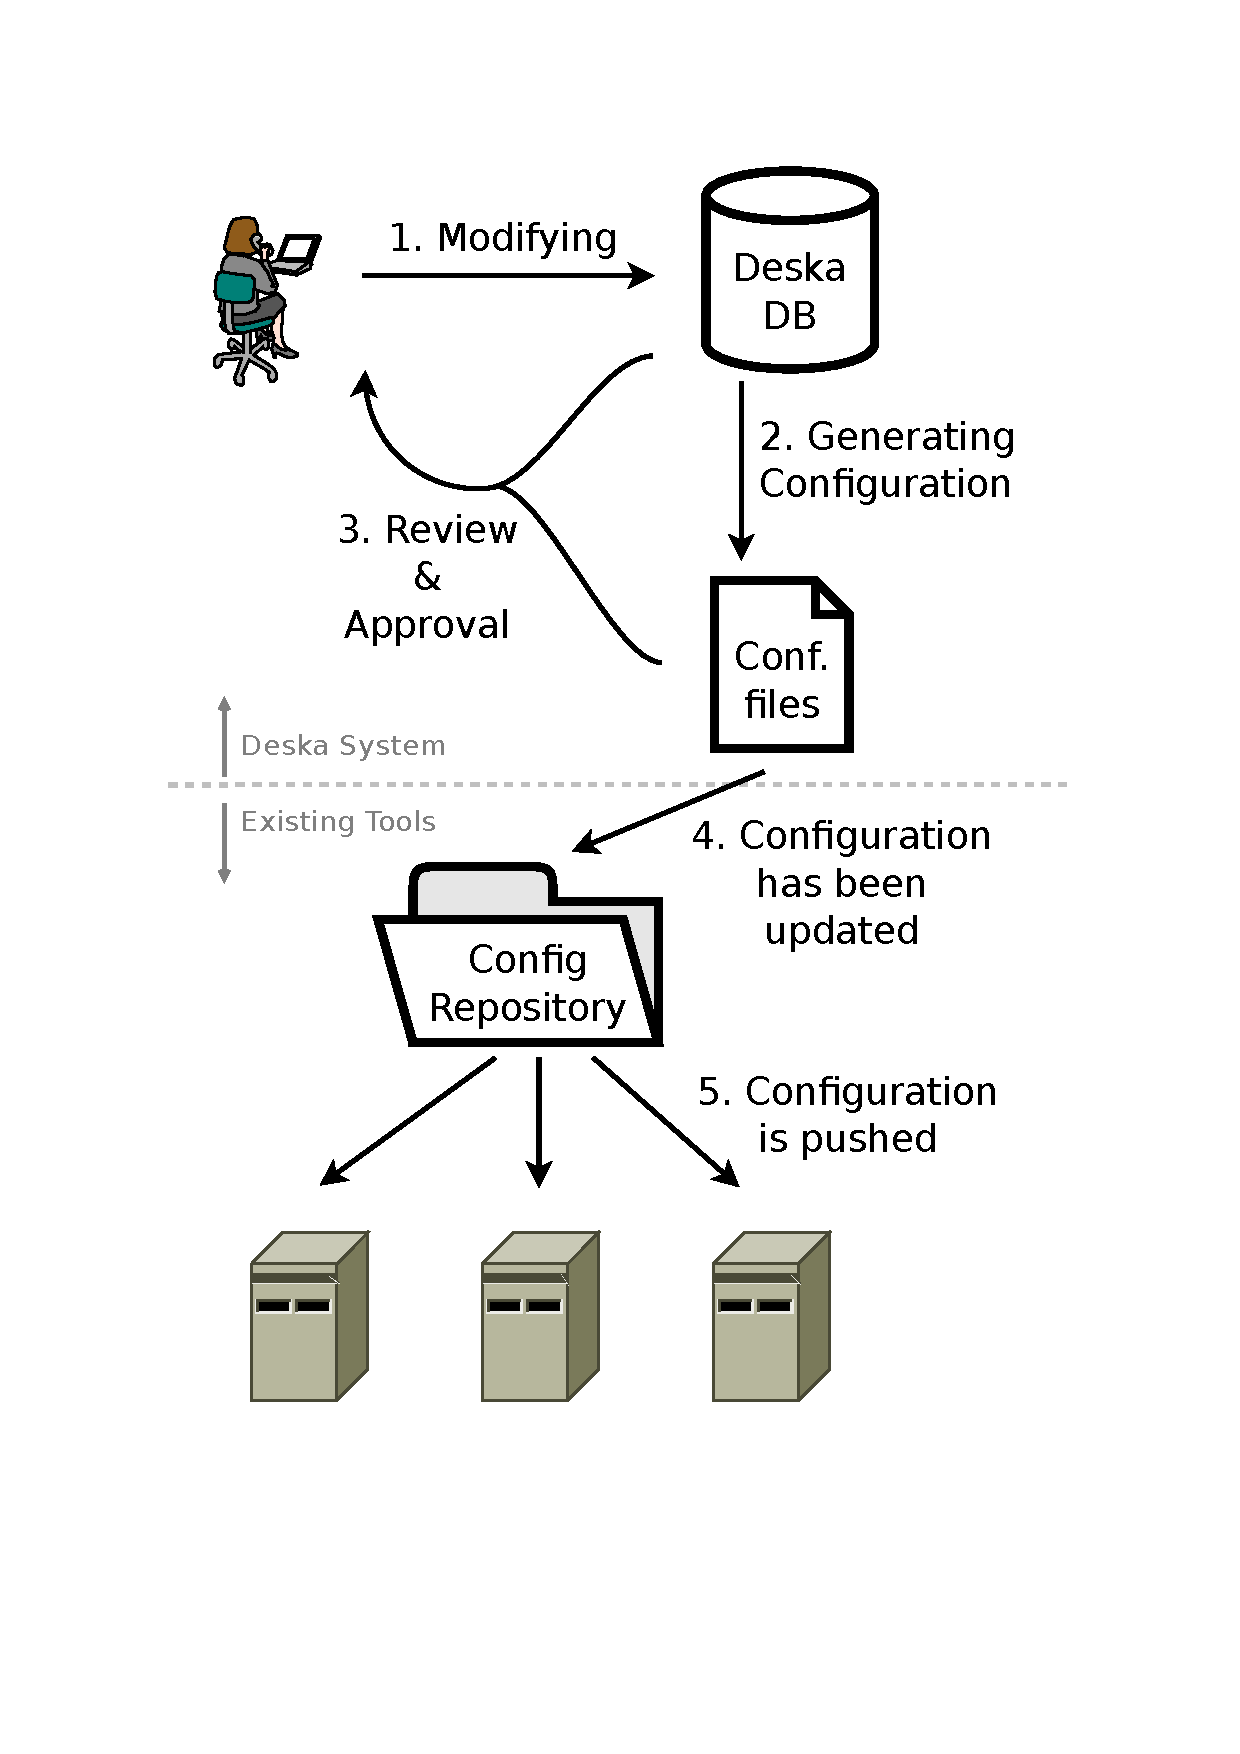
\includegraphics[height=90mm, trim=28mm 53mm 30mm 28mm, clip=true]{../../technical/img-deska-workflow.pdf}
\end{textblock}
\end{column}
\end{columns}
\end{frame}


\begin{frame}[fragile]
\begin{center}
Ukázka práce na FZÚ
\end{center}
% The goal here is to show how a small change in the database affects the generated output and how one can review the
% data.
% - Working with the d_fzu DB which contains a production snapshot of the FZU database (straight from the dump)
% - Mention the heavy tab completion?
% - `host golias111
% - `show`
% - `interface [Tab]`, doplneni eth0
% - `start`
% - `diff`
% - `configdiff`
% - comment on a single change in the Deska DB contents having a big impact on the output
% - maybe mention that the subsequent runs are instant
% - also add a note that Deska is just one out of *many* users of the Git repo and that it doesn't matter that others
%   are making changes at the same time
\end{frame}


\begin{frame}[fragile]
\frametitle{Požadavky zadavatele}
\begin{itemize}
    \item CLI rozhraní
    \item WWW přístup není požadován
    \item Skriptování
    \item Verzování, audit logging
    \item Izolované změny --- sandbox
    \item Preference FLOSS, Linux
    \item Integrace s existující infrastrukturou
    \item Nevynalézat znovu kolo
\end{itemize}
\end{frame}


\begin{frame}[fragile]
\frametitle{Struktura databáze}
\begin{itemize}
    \item Dynamické požadavky, každé centrum trochu jiné
        \begin{itemize}
            \item Generická databáze
            \item Schéma dotváří správce aplikace
        \end{itemize}
    \item Implementace
        \begin{itemize}
            \item SQL DDL jako definice schématu
            \item Generátory kódu pro uložené procedury
        \end{itemize}
    \item Zapouzdření
        \begin{itemize}
            \item Klientské aplikace {\em nezávislé} na schématu
            \item Komunikační protokol schopný popsat uživatelské schéma
            \item Introspekce
        \end{itemize}
\end{itemize}
\end{frame}


\begin{frame}[fragile]
\frametitle{Databázová struktura: objekty}
\begin{itemize}
    \item Každá položka reprezentovaná {\bf objektem} patřičného typu (``kind'')
        \begin{itemize}
            \item {\bf Kind} $\rightarrow$ databázová tabulka
                \begin{itemize}
                    \item Určuje povolené atributy a jejich datové typy
                    \item {\tt hardware}, {\tt switch}, {\tt vendor},\ldots
                \end{itemize}
            \item {\bf Objekt} $\rightarrow$ řádka v~tabulce
                \begin{itemize}
                    \item ({\tt wn123}, {\tt www01}, {\tt wn123->eth0}, {\tt Cisco},\ldots)
                \end{itemize}
        \end{itemize}
        \begin{minted}{text}
            host wn123
                hardware sgi-xe310
                rack R06
                position 10
            end
        \end{minted}
    \item Schéma je uživatelsky definováno
        \begin{itemize}
            \item Deska server neobsahuje nic specifického pro datacentrum
        \end{itemize}
\end{itemize}
\end{frame}


\begin{frame}[fragile]
\frametitle{Databázová struktura: relace}
\begin{itemize}
    \item Relace určují pravidla pro vztahy mezi jednotlivými tabulkami
    \item Přidání konkrétního {\em významu} cizím klíčům
        \begin{itemize}
            \item {\bf Odkazování}
                \begin{itemize}
                    \item Odkaz na patřičný {\tt vendor} z~každého {\tt hardware}
                \end{itemize}
            \item {\bf Tagování}
                \begin{itemize}
                    \item Přiřazení logických rolí jednotlivým serverům
                \end{itemize}
            \item {\bf Template} určuje výchozí hodnotu atributů
                \begin{itemize}
                    \item Dodávka mnoha serverů najednou
                \end{itemize}
            \item Objektová {\bf kompozice}
                \begin{itemize}
                    \item Opětovné využití subkomponent -- {\tt server} i {\tt switch} jsou v~{\tt rack}u
                \end{itemize}
            \item {\bf Vnořování} objektů
                \begin{itemize}
                    \item Umožňuje vytvářet hierarchické stromy objektů modelující realitu
                    \item Síťová rozhraní: {\tt srv123->eth0}
                \end{itemize}
        \end{itemize}
\end{itemize}
\end{frame}


\begin{frame}[fragile]
\frametitle{Technická implementace}
\begin{columns}
\begin{column}{.45\paperwidth}
    \begin{itemize}
        \item Klient-server aplikace
            \begin{itemize}
                \item 100\% oddělení
            \end{itemize}
        \item Klient:
            \begin{itemize}
                \item CLI
                \item C++, Boost, Spirit
                \item komunikace přes JSON, SSH
            \end{itemize}
        \item Server:
            \begin{itemize}
                \item PostgreSQL~9.0
                \item Pl/PgSQL, PgPython
                \item generátory kódu
                \item Python pomocné funkce
            \end{itemize}
        \item Výstupní generátory:
            \begin{itemize}
                \item Python
                \item nativní přístup k~DB objektům
                \item Git
            \end{itemize}
    \end{itemize}
\end{column}
\begin{column}{.55\paperwidth}
\begin{textblock}{50}(0,-7.5)
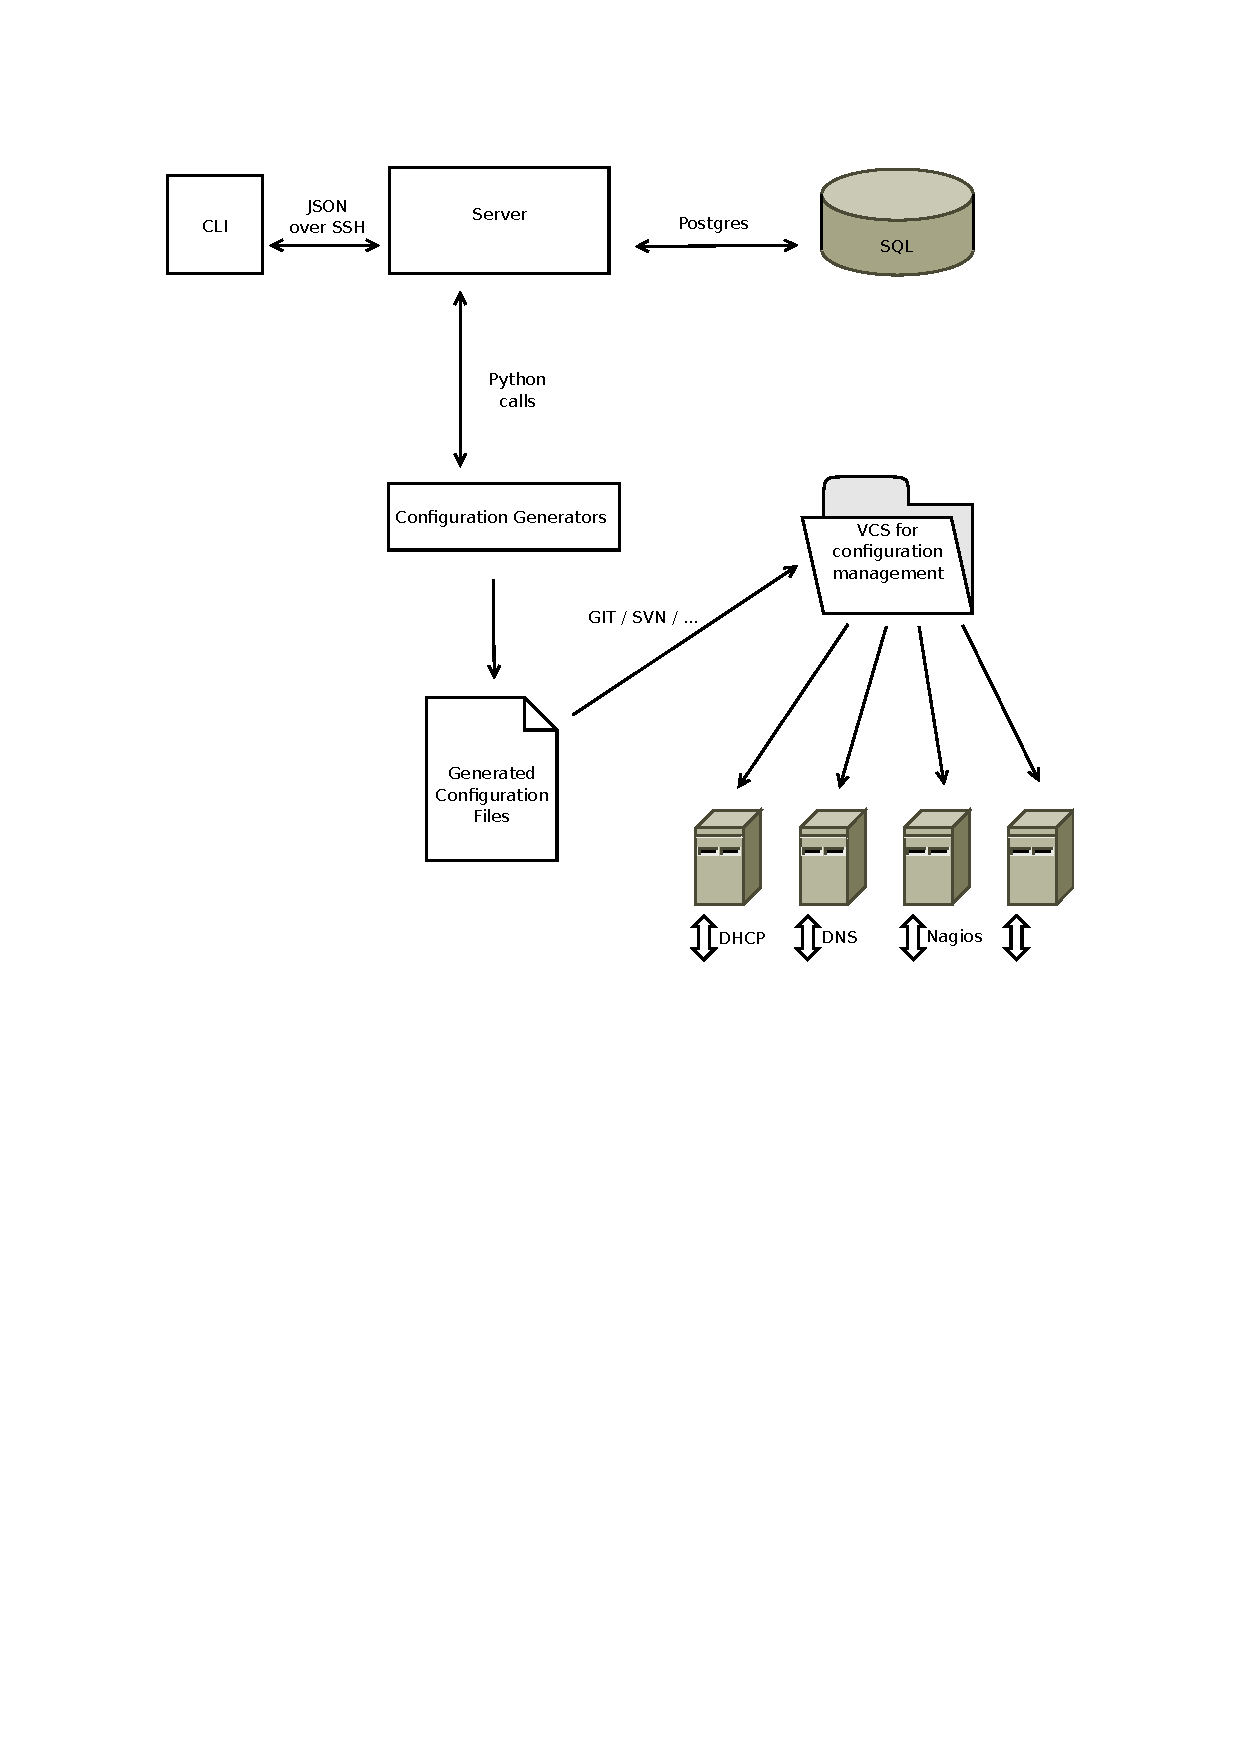
\includegraphics[width=65mm, trim=28mm 64mm 28mm 27mm, clip=true]{../../technical/img-deska-components.pdf}
\end{textblock}
\end{column}
\end{columns}
\end{frame}


\begin{frame}[fragile]
\frametitle{Skriptování v Pythonu}
\begin{itemize}
    \item Zpřístupnění obsahu databáze přes nativní objekty
        \begin{itemize}
            \item Vytvoření hierarchie tříd za~běhu
            \item Introspekce přes oficiální komunikační protokol
            \item Čistě automatický proces
        \end{itemize}
    \item Filtrování probíhá na straně serveru
    \item Syntaxe podobná standardnímu ORMu SQL Alchemy
\end{itemize}
\begin{minted}{python}
import deska
# introspekce
deska.init()

for host in deska.host[(deska.host.color == "red") &
                       deska.service.contains("www")]:
    print "%s\n" % host
\end{minted}
\end{frame}


\begin{frame}[fragile]
\begin{center}
Předvedení Desky
\end{center}
% start with the DEMO scheme
%   `dump`, `log`, `resume`: everything is empty (r1 is a system revision)
% Let's start a changeset so that we can perform modifications:
%   start
% Let's add a first object to the database.  Use tab completion:
%   create vendor HP
% See that it got added:
%   dump
% And the database does show it in the diff:
%   diff
% Let's create our first server. We're going to use another syntax now:
%   hardware srv123
% We've now switched to another context.  Let's try making clear that it's an HP server.
% Again, we're going to use Tab completion heavily, both for "vendor" *and* the "HP":
%   vendor HP
% Let's see what we've done and try to commit the data. This is going to fail:
%   commit blah
% OK, it says that we shall add some non-NULL data. Fair enough:
%   purchase 2011-01-01
%   diff
% Let's call it finished:
%   commit Initial data
% We're back in the root context and our data are saved:
%   dump
% Create another vendor and another server:
%   create vendor IBM
%   hardware pc02
%   purchase 1998-10-01
%   vendor IBM
%   end
% Commit these changes:
%   commit
% Get back to work now:
%   start
% Pretend that the vendor got removed:
%   rename vendor IBM Lenovo
% The diff shows the rename just at one place, *not* for the hardware:
%   diff
% Save the data:
%   commit IBM got bought
% Try to create an inconsistency in the DB:
%   delete vendor Lenovo
%   diff
% You cannot save such a changeset:
%   commit
%   abort
% Introduce a first template:
%   start
%   hardware_template old_ibm_box
%   vendor Lenovo
%   warranty 2005-12-31
% See? The required ``purchase'' is not there, and it doesn't matter -- it's just a template.
%   diff
%   commit
% Try to make use of the template:
%   start
%   hardware ibm01 template_hardware old_ibm_box
%   hardware ibm02 template_hardware old_ibm_box
%   hardware ibm03 template_hardware old_ibm_box
% Try a commit, but it will fail:
%   commit
% Let's change the data just at a single place, then:
%   hardware_template old_ibm_box purchase 1995-01-01
% The diff tries to be smart and shows just that single change here:
%   diff
%   commit
%   diff r5 r6
% Again, the diffs are compact. OTOH, the `show` command shows everything correctly:
%   show hardware ibm01
% The same for `dump` which is also meant for human consumption. OTOH, backup is correct:
%   backup filename
% Demonstrate how to restore from backup:
%   [run the reinstallation here]
%   ./deska-cli
% Tab completion works even for filenames:
%   restore filename
% The data are properly restored:
%   log
%   log (vendor == HP)
%   log (hardware == ibm01)
%   diff rSomething
% See the filters in action:
%   hardware where (vendor == Lenovo)
%   context objects
% Try to do a mass-modification:
%   note_hardware blabla
%   diff
%   commit
%   diff
% Move to the contained/containable objects:
%   host srv123
%   diff
% The diff shows that the objects are linked together -- as automated by the Deska DB.
% Try to make a mistake, create a virtual_hw:
%   vram 4
%   commit fail
%   end
%   delete virtual_hardware srv123
% Adding some services to the mix:
%   create service www
%   create service ftp
%   host srv123
%   add service www
%   add service ftp
%   commit
%   diff
% Setting services works even in an absolute way:
%   host srv123
%   service [www]
%   diff
%   commit
%   diff
% Create an interface, set an IPv4 address, show how is the embedding reflected in the CLI's show/dump
% Demonstrate rebase using hardware's attributes, maybe combine with some mass-setAttribute calls

\end{frame}


\begin{frame}[fragile]
\frametitle{Problémy v použitých komponentách}
\begin{itemize}
    \item PostgreSQL: nedostatečná chybová diagnostika u selhávajících integritních omezení
        \begin{itemize}
            \item náš patch zařazen do PostgreSQL 9.2
            \item nabídka zaměstnání v~evropské společnosti
        \end{itemize}
    \item Boost.Process: špatné ošetření návratových hodnot syscallů {\tt read(2)}, {\tt write(2)}
        \begin{itemize}
            \item neoficiální knihovna, není součástí Boostu
            \item opraveno lokálně, další rozšíření funkčnosti
        \end{itemize}
    \item JSON-Spirit: serializace floating-point čísel neodpovídá specifikaci JSONu
        \begin{itemize}
            \item patch
        \end{itemize}
    \item PsycoPg2: porušení zpětné kompatibility mezi verzemi 2.4.2 a 2.4.1
        \begin{itemize}
            \item workaround, podporujeme všechny rozšířené verze
        \end{itemize}
    \item PgPython: nedostatečné rozlišování prázdných polí a prázdných řetězců, nedostatečná kontrola chyb
        \begin{itemize}
            \item workaround
        \end{itemize}
    \item CMake/CDash: integrace s~Redmine
        \begin{itemize}
            \item patch
        \end{itemize}
\end{itemize}
\end{frame}


\begin{frame}[fragile]
\frametitle{Nasazení na FZÚ}
\begin{itemize}
    \item Deska nasazena v pilotním provozu
        \item Generování reálných výstupů pro produkční služby
        \begin{itemize}
            \item Nagios
            \item Munin
            \item cfengine
            \item Bind (DNS)
            \item DHCP
            \item Ethernetové přepínače
            \item Ganglia
        \end{itemize}
    \item Vizualizace serverovny (QML)
\end{itemize}
\end{frame}

\begin{frame}[fragile]
\frametitle{Statistika}

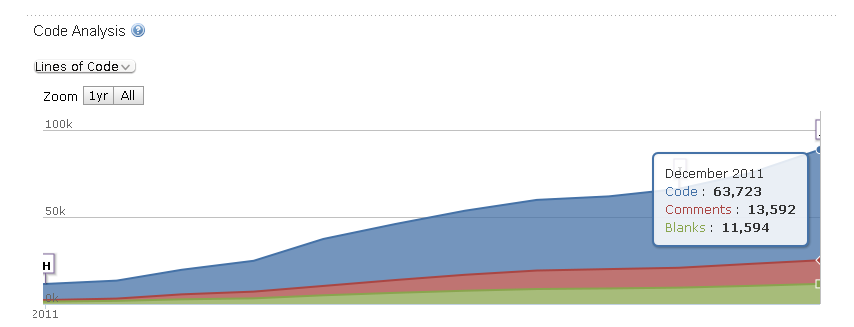
\includegraphics[width=\textwidth]{deska-ohloh-loc-2011.png}

\begin{columns}[t]
\begin{column}{.45\textwidth}
\begin{itemize}
    \item 750+ odpracovaných hodin za~jednoho člena týmu
    \item Nejrozsáhlejší komponenta: {\bf testy}
\end{itemize}
\end{column}
\begin{column}{.6\textwidth}
\begin{itemize}
    \item Celkové náklady (Basic~COCOMO, Organic~Project):
        \begin{description}
            \item[člověkoroky] 9,7
            \item[počet vývojářů] 7,64
            \item[odhadovaná doba] 15,24 měsíců
        \end{description}
\end{itemize}
\end{column}
\end{columns}
\end{frame}




\begin{frame}[fragile]
\frametitle{Shrnutí}
\begin{itemize}
    \item Generická databáze
        \begin{itemize}
            \item Práce nad uživatelským schématem
            \item Verzování
        \end{itemize}
    \item Splňuje podmínky k produkčnímu nasazení, ověřeno v~pilotním provozu
    \item Řeší reálné požadavky uživatelů
    \item Patche přijaty open-source projekty
    \item Automatizované testy na mnoha úrovních
    \item Vystoupení na třech zahraničních konferencích (Dubna, Taipei, Vancouver)
        \begin{itemize}
            \item dvě publikace, jedna recenzovaná v~Journal of Physics
        \end{itemize}
\end{itemize}
\end{frame}


\begin{frame}[fragile]
\frametitle{Dotazy}
\begin{center}
    Děkujeme za pozornost
\end{center}
\end{frame}

\end{document}
